\documentclass[conference]{IEEEtran}
\usepackage{times}

\usepackage{amsmath}
\usepackage{amsopn}
\DeclareMathOperator*{\argmin}{\arg\!\min} 
\DeclareMathOperator*{\argmax}{\arg\!\max} 

\usepackage{graphicx}
\usepackage{caption}
\usepackage{subcaption}
% numbers option provides compact numerical references in the text. 
\usepackage[numbers]{natbib}
\usepackage{multicol}
\usepackage[bookmarks=true]{hyperref}

\pdfinfo{
   /Author (Homer Simpson)
   /Title  (Robots: Our new overlords)
   /CreationDate (D:20101201120000)
   /Subject (Robots)
   /Keywords (Robots;Overlords)
}

\begin{document}

% paper title
\title{Inverse Reinforcement Learning from Failure}

% You will get a Paper-ID when submitting a pdf file to the conference system
\author{Kyriacos Shiarlis, Joao Messias, Maarten Van Someren, Shimon Whiteson}

%\author{\authorblockN{Michael Shell}
%\authorblockA{School of Electrical and\\Computer Engineering\\
%Georgia Institute of Technology\\
%Atlanta, Georgia 30332--0250\\
%Email: mshell@ece.gatech.edu}
%\and
%\authorblockN{Homer Simpson}
%\authorblockA{Twentieth Century Fox\\
%Springfield, USA\\
%Email: homer@thesimpsons.com}
%\and
%\authorblockN{James Kirk\\ and Montgomery Scott}
%\authorblockA{Starfleet Academy\\
%San Francisco, California 96678-2391\\
%Telephone: (800) 555--1212\\
%Fax: (888) 555--1212}}


% avoiding spaces at the end of the author lines is not a problem with
% conference papers because we don't use \thanks or \IEEEmembership


% for over three affiliations, or if they all won't fit within the width
% of the page, use this alternative format:
% 
%\author{\authorblockN{Michael Shell\authorrefmark{1},
%Homer Simpson\authorrefmark{2},
%James Kirk\authorrefmark{3}, 
%Montgomery Scott\authorrefmark{3} and
%Eldon Tyrell\authorrefmark{4}}
%\authorblockA{\authorrefmark{1}School of Electrical and Computer Engineering\\
%Georgia Institute of Technology,
%Atlanta, Georgia 30332--0250\\ Email: mshell@ece.gatech.edu}
%\authorblockA{\authorrefmark{2}Twentieth Century Fox, Springfield, USA\\
%Email: homer@thesimpsons.com}
%\authorblockA{\authorrefmark{3}Starfleet Academy, San Francisco, California 96678-2391\\
%Telephone: (800) 555--1212, Fax: (888) 555--1212}
%\authorblockA{\authorrefmark{4}Tyrell Inc., 123 Replicant Street, Los Angeles, California 90210--4321}}


\maketitle

\begin{abstract}
In this paper, we approach the problem of Inverse Reinforcement Learning (IRL) from a rather different perspective. Instead of trying to only mimic an expert as in 
traditional IRL, we present a method that can utilise information from failed or bad demonstrations of a task. To this end, we derive a new IRL algorithm that extends the state-of-the-art method of Maximum Causal Entropy Inverse Reinforcement Learning.  Futhermore, we present experimental results showing that our method can converge faster and learn better than its original counterpart, at no extra computational cost. 
\end{abstract}

\IEEEpeerreviewmaketitle

\section{Introduction and Motivation}
Inverse reinforcement Learning (IRL) has been subject to a significant amount of research since its introduction to the computer science research community by Ng and Russel \cite{ng2000algorithms}. The problem involves an agent or \emph{apprentice} acting in an environment modelled by a Markov Decision Process (MDP) for which the reward function is not available but samples from the policy of an \emph{expert} performing the decision-making, are given instead. An IRL algorithm tries to find a reward function that allows the apprentice to exhibit similar behaviour as the expert and generalises well to situations for which data is not available. The IRL formulation is particularly appealing in Markovian Decision Tasks for which the actual reward function is very difficult to define explicitly, but examples of correct behaviour can be generated instead. For this exact reason the main applications of the method have been in simulated car driving[] and socially appropriate navigation\cite{henry2010learning}\cite{vasquez2014inverse}. To achieve this researchers have  adapted concepts from the wider Machine Learning community, like maximum entropy\cite{ziebart2008maximum} and bayesian formulations \cite{ramachandran2007bayesian}, structured classification \cite{ratliff2006maximum}, boosting \cite{ratliff2007boosting} and gaussian processes\cite{levine2011nonlinear} with varying degrees of success.\\

Despite its appealing applications and encouraging research the IRL framework still suffers from a number of important theoretical and practical drawbacks. Firstly, because of their iterative nature most known methods require solving an MDP under the current reward before an update. For large state spaces, Markov decision processes becomes prohibitive to evaluate once, let alone a number of times. Secondly, most algorithms are non-convex in nature especially if the dynamics of the system are non-deterministic and ill posed how do I make the differentiation? More practical issues include generalisation, if the observed expert's behaviour is too limited, it is very hard to generalise to new parts of the state space, especially if this is too large. In addition, since the expert can be expected to avoid punishing states, information about the reward in these states reaches us only implicitly, making generalisation of the reward function an even harder task. \\

We present the first step towards allowing IRL algorithms to leverage a wider variety of data to learn faster and generalise better. Specifically we consider the case where appart from
an Expert dataset we have access to a dataset of behaviour that should be avoided at all costs. Our algorithm tries to approach the expert behaviour at while avoiding the failed trajectories.

This altered view of IRL emerges from the basic principle that governs most IRL algorithms. Because the observed data is assumed to be coming from an Expert, IRL tries to make the value of the observed trajectories optimal by tweeking the reward function in an intelligent way, most commonly by gradient (or subgradient) descent. We can imagine however that we observe a certain trajectory in the state space and we have access to an annotator that can tell us to what \emph{degree} the observe behaviour is optimal. If for example we observe the worst possible behaviour, then we can possibly demand from our algorithm to \emph{minimise} value for those trajectories when generated by the apprentice. Importanly, this view preserves the main motivation for IRL which is that the reward function for each state-action pair need not be hardcoded, while \emph{extending} the scope from which demonstrations can be considered useful to learning. In addition, by exploiting the information contained within, for example, failed trajectories, we gain access to more explicit information about the nature of the reward at certain areas of the state-space that the expert could only implicitly provide. This provides additional constraints to combat the aforementioned illposition of IRL and allow's us to build reward functions that are more likely to generalise to unseen situations. Finally such a framework would allow the designer to inject prior knowledge into the learning process in a principled manner, without the need for complex prior distributions and extra computational cost. If we are previously aware of parts of the state-space that should have a very negative reward, we can (assuming the dynamics are known) simulate data of the agent acting in an environment where large rewards are given for reaching unwanted states. Feeding our generated data along with that of the expert into our extended IRL algorithm would allow the apprentice to imitate the expert while learning a reward function that takes into account our domain knowledge.



\section{Method Outline}
	In his PhD thesis Ziebart after introducing the principle of Maximum Causal Entropy he applies it to generalised Inverse Optimal Control(IOC) and IRL by assuming an agent acting in an MDP. The model is very powerful, easy to apply and results in a convex optimisation problem. In its heart, the algorithm tries to find the stochastic policy $\pi(a|s)$ that maximises the causal entropy of an influence model of a certain time duration $T$ while constrained to match certain statistics from the expert dataset $\mathcal{D}$. These statistics are called the empirical feature expectations $\widetilde{\Phi}_{\mathcal{D}}$. The optimisation is solved using Lagrangian multipliers and results in a procedure very similar to most IRL methods. A policy
	is found under the current reward function using a 'soft' version of the Bellman equations, the feature expectations of the model are then calculated from the initial  states in the data, and finally a reward update step based on the comparison between the empirical and model feature expectations.\\
	Our method directly modifies this optimization process in two significant ways. Firstly using a set of slacks we call $\zeta^+$ and $\zeta^-$ we relax the feature matching constraint between the emodel and the expert data. Instead we demand that the value of these slacks is minimised. Secondly we intoduce a second set of constraints that aim to create disimilarity between the model feature expecations and those of a dataset of failed demonstrations $\widetilde{\Phi}_{\mathcal{D}_b}$. This is done through a second set of slacks $\alpha^+$ and $\alpha^-$ that we aim to \emph{maximise}. These modifications results in the following optimisation problem.
	
	\begin{equation}
	\argmax_{\pi(a,s),\alpha^+_k ,\alpha^-_k ,\zeta^+_k, \zeta^-_k} H(\mathbf{A}^T||\mathbf{S}^T) - \sum_k\big(C(\zeta^+_k + \zeta^-_k)  -D(\alpha^+_k  \alpha^-_k)\big)
\end{equation}
\begin{equation}
	\widetilde{\Phi}_{\mathcal{D},k}-\Phi_{\pi,s_0,k}   = \zeta^+_k  - \zeta^-_k \quad \forall k \label{eq:good_ineq}
\end{equation}
\begin{equation}
	\widetilde{\Phi}_{\mathcal{D}_b,k}-\Phi_{\pi,s_0,k}  = \alpha^+_k-\alpha^-_k \quad \forall k \label{eq:bad_ineq}
\end{equation}
\begin{equation}
	-\zeta^+_k \leq 0 \quad \text{and} \quad -\zeta^-_k \leq 0 \quad \forall k
\end{equation}
\begin{equation}
	-\alpha^+_k \leq 0 \quad \text{and} \quad -\alpha^-_k \leq 0 \quad \forall k
\end{equation}
\begin{equation}
	\alpha^-_k \alpha^+_k = 0 \quad \forall k  \label{eq:quadratic}
\end{equation}
\begin{equation}
	\text{and:   }\sum_aP(a|s)  = 1 \quad \forall s  
\end{equation}
\begin{equation}
	\text{and:   }P(a|s)  > 0 \quad \forall s,a  
\end{equation}


\section{Experiments and Results}
We perform experiments on "moving obstacle gridworld". In much the same spirit as the original toy problem an agent tries to reach a target square (T) of very high reward,
while avoiding some squares of negative reward(N). The only difference is that the (N)  squares are moving in different directions at every time step. This was done to closer simulate robotic navigation towards a target while avoiding a moving person. For proof-of-concept purposes the test problem is fully deterministic. We demonstrate the performance of our method by directly comparing it to the original algorithm as described by Ziebart. \\
%
%To begin comparison between the two methods we first need some synthetic data from the problem, or at least the two quantities $\widetilde{\Phi}_{\mathcal{D},k}$ and $\widetilde{\Phi}_{\mathcal{D}_b,k}$ for the good and bad datasets repsectively. These can be generated very easily using the forward algorithm also given by Ziebart, using a policy P(a|s), model dynamics and an initial state distribution $b_{0,train}$. The policies in turn arise from two reward functions $R_e$ for the expert and $R_t$ for the taboo-agent. 

Firstly we generate synthetic feature expectations $\widetilde{\Phi}_{\mathcal{D},k}$ for the expert and $\widetilde{\Phi}_{\mathcal{D}_b,k}$ for the taboo agent as they arise by allowing these agents to start from an initial state distribution $b_{0,train}$ and proceed for $T$ timesteps under their 'soft' optimal policies that result from their respective reward functions $R_e$ and $R_t$. Using this data we train two apprentices, one that only considers data from the expert, using the original algorithm and another that considers both sets of data, using our extended method. The evaluation of the two algorithms is done using a test distribution of initial states $b_{0,test}$ in order to assess the ability of the learned Reward functions to generalise to new initial conditions. The evaluation is done based on three metrics namely:

		We evaluate the toy problem based on three initial criteria:
			\begin{itemize}
				\item The value accumulated by the apprentice in T timesteps starting from $b_{0,test}$ when evaluated on the experts reward function, $R_e$. If the apprentice achieves similar Value accumulation as the expert, it means that the trajectories executed by the two agent's are similar.

				\item The value accumulated by the apprentice in N timesteps from a test initial state distribution $b_{0,test}$ when evaluated on the initial taboo agents reward function $R_t$. The less Value is accumulated here, the better since we want to perform badly on the taboo-agents reward function.
				\end{itemize}
	
	Figure \ref{fig:res} demonstrates the results from our experiments. In \ref{fig:res_a} we can see that our algorithm (blue) acumulates as much value as the expert (black line) while the original algorithm (red) does not converge in the given amount of iterations. Turning to \ref{fig:res_b}, the green line represents the value accumulated by the expert based on the taboo agents reward function. We can see that our algorithm can do even worse than the expert on the taboo agents reward while original algorithm doesn't.

\begin{figure}[t]
  \centering
  \begin{subfigure}[b]{0.5\textwidth}
    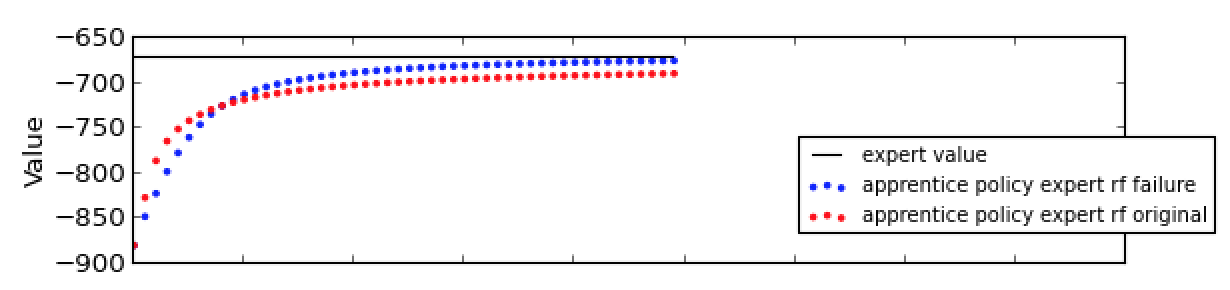
\includegraphics[scale=0.4]{resa}
    \caption{Expert Reward Function}
    \label{fig:res_a}
  \end{subfigure}
  \begin{subfigure}[b]{0.5\textwidth}
    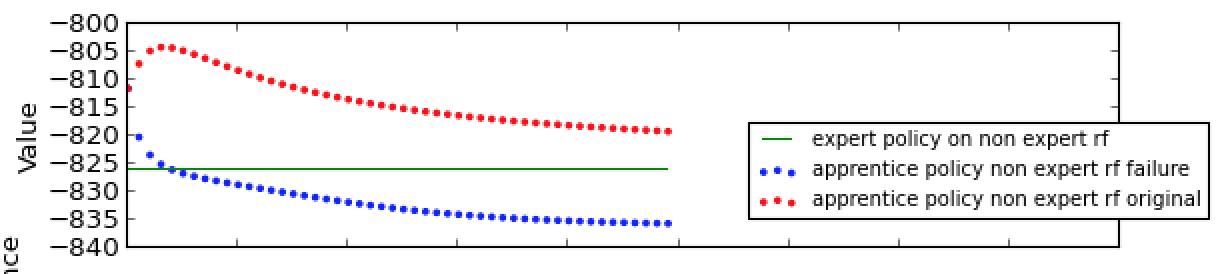
\includegraphics[scale=0.4]{resb.png}
        \caption{Taboo Reward Function}
    \label{fig:res_b}
\end{subfigure}
  \caption{Results from Moving obstacle gridworld experiments. Our algorithm (blue) surpasses the original (red) in both imitating the expert and not imitating the taboo agent}
  \label{fig:res}
\vspace{-4mm}
\end{figure}


These results demonstrate that taking into account failed demonstrations of a task will allow the apprentice to generalise better to new initial states and learn in fewer iterations than previously possible.

\section{Conclusions and further work}
	We have demonstrated the merits of allowing IRL algorithms to go beyond expert demonstrations to demonstrations of varying value. We further demonstrated an instance of such a modified algorithm that can learn better and in fewer iterations than its original counterpart. Our immediate future work involves applying these methods to more realistic scenarios such as simulated and real life robots. Another very interesting direction that we will pursue is how the similarity between the expert and taboo datasets affect the ability to learn. Finally we would like to extend our modifications to other popular IRL algorithms.
%Proof of concept that failed trajectories contain valuable information for learning in many fronts. 
%Further work includes:
%\begin{itemize}
%	\item Tackling problems of having very similar data from expert and non expert.
%	\item Applying concept to other methods that might require different treatment.
%\end{itemize}
%
%
%\section{RSS citations}
%
%Please make sure to include \verb!natbib.sty! and to use the
%\verb!plainnat.bst! bibliography style. \verb!natbib! provides additional
%citation commands, most usefully \verb!\citet!. For example, rather than the
%awkward construction 
%
%{\small
%\begin{verbatim}
%\cite{kalman1960new} demonstrated...
%\end{verbatim}
%}
%
%\noindent
%rendered as ``\cite{kalman1960new} demonstrated...,''
%or the
%inconvenient 
%
%{\small
%\begin{verbatim}
%Kalman \cite{kalman1960new} 
%demonstrated...
%\end{verbatim}
%}
%
%\noindent
%rendered as 
%``Kalman \cite{kalman1960new} demonstrated...'', 
%one can
%write 
%
%{\small
%\begin{verbatim}
%\citet{kalman1960new} demonstrated... 
%\end{verbatim}
%}
%\noindent
%which renders as ``\citet{kalman1960new} demonstrated...'' and is 
%both easy to write and much easier to read.
%  
%\subsection{RSS Hyperlinks}
%
%This year, we would like to use the ability of PDF viewers to interpret
%hyperlinks, specifically to allow each reference in the bibliography to be a
%link to an online version of the reference. 
%As an example, if you were to cite ``Passive Dynamic Walking''
%\cite{McGeer01041990}, the entry in the bibtex would read:
%
%{\small
%\begin{verbatim}
%@article{McGeer01041990,
%  author = {McGeer, Tad}, 
%  title = {\href{http://ijr.sagepub.com/content/9/2/62.abstract}{Passive Dynamic Walking}}, 
%  volume = {9}, 
%  number = {2}, 
%  pages = {62-82}, 
%  year = {1990}, 
%  doi = {10.1177/027836499000900206}, 
%  URL = {http://ijr.sagepub.com/content/9/2/62.abstract}, 
%  eprint = {http://ijr.sagepub.com/content/9/2/62.full.pdf+html}, 
%  journal = {The International Journal of Robotics Research}
%}
%\end{verbatim}
%}
%\noindent
%and the entry in the compiled PDF would look like:
%
%\def\tmplabel#1{[#1]}
%
%\begin{enumerate}
%\item[\tmplabel{1}] Tad McGeer. \href{http://ijr.sagepub.com/content/9/2/62.abstract}{Passive Dynamic
%Walking}. {\em The International Journal of Robotics Research}, 9(2):62--82,
%1990.
%\end{enumerate}
%%
%where the title of the article is a link that takes you to the article on IJRR's website. 
%
%
%Linking cited articles will not always be possible, especially for
%older articles. There are also often several versions of papers
%online: authors are free to decide what to use as the link destination
%yet we strongly encourage to link to archival or publisher sites
%(such as IEEE Xplore or Sage Journals).  We encourage all authors to use this feature to
%the extent possible.
%\section*{Acknowledgments}

%% Use plainnat to work nicely with natbib. 

\bibliographystyle{plainnat}
\bibliography{references}

\end{document}


